\subsection{Performances}
\label{sec:perf}
Outre son aspect algorithmique qui permet des paramétrages particuliers, XGBoost a également été conçue pour être une méthode d'apprentissage performante du point de vue de l'utilisation des ressources et de la parallélisation.
\subsubsection{Optimisations réalisées}
\subParagraphe{Parallélisation}Comme nous l'avons expliqué en Section~\ref{sec:gradient-boosting}, XGBoost va entraîner des arbres au fur et à mesure pour améliorer une métrique. Ainsi, il n'est pas possible de paralléliser l'entraînement des arbres, puisque l'arbre $n$ va dépendre des arbres entraînés précédemment (que ce soit sur l'échantillon ou le poids des données).

Cependant, XGBoost se démarque en proposant à la place une solution pour paralléliser la création d'arbre en calculant des branches de manière indépendante.
\subParagraphe{Mémoire}
\subParagraphe{Utilisation du cache}
\subParagraphe{Conception}
\subParagraphe{Externalisation des données}
\subsubsection{Benchmarking des solutions}
Plusieurs études ont été menée pour comparer les performances de XGBoost vis-à-vis d'autres solutions.
\subParagraphe{Benchmarking par Tong~\textsc{He}}Le créateur de XGBoost a réalisé un comparatif de temps d'exécution entre son algorithme et d'autres algorithme courants sur le challenge Kaggle du boson de Higgs~\cite{bib:boson}. Les résultats de ce benchmarking sont repris à la Figure~\ref{fig:perfun}.

\begin{figure}[h]
	\begin{margincap}
		\centering
		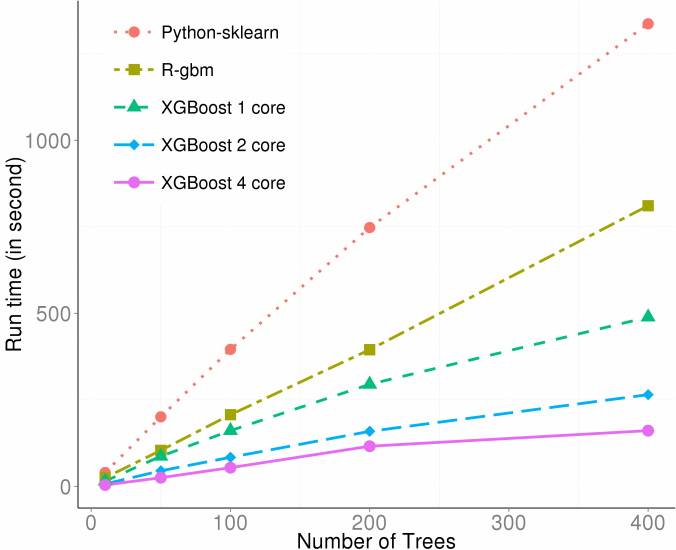
\includegraphics[width=.6\textwidth]{images/More/perf_un}
		\caption{Comparaison des temps d'apprentissage entre XGBoost et d'autres algorithmes importants de Machine Learning sur le challenge Kaggle du boson de Higgs}
		\label{fig:perfun}
	\end{margincap}
\end{figure}

Sur la Figure~\ref{fig:perfun}, les courbes \textit{Python-sklearn} et \textit{R-gbm} correspondent à des algorithmes GBM déjà existants sur ces plateformes, alors que XGBoost correspond à des essais avec l'algorithme nouvellement développé. L'influence du nombre de c\oe urs utilisés est également testé ici (tous les apprentissages se font à même paramétrage). On tire de ce graphe les conclusions suivantes :\begin{itemize}
\itemperso{XGBoost et autres GBM}Mis à part pour un faible nombre d'arbres appris, XGBoost obtient des performances de bien meilleures (deux fois plus rapide) que les autres solutions de GBM.
\itemperso{Influence du nombre de c\oe ur}Plus le nombre de c\oe urs pour paralléliser XGBoost est important, plus ce dernier est rapide, même si on observe un tassement passé quatre c\oe urs\mysidenote{Ceci est logique, car comme nous l'avons vu, il n'est pas possible de paralléliser tout le processus d'apprentissage, mais seulement une partie de ce dernier. Ainsi, il restera une partie que l'on ne peut réduire, d'où ce constat.}.
\end{itemize}

\subsubsection{Benchmarking par rapport à des implémentations de Random Forest}
Un autre Benchmarking a également visé à comparer les performances de XGBoost 
